\chapter{Development of the Interferometer}
\thispagestyle{empty}
With the software implementation completed, all components required for the interferometric measurements were available. This chapter presents the complete experimental setup used throughout this work.

\section{Experimental Setup}

 The interferometer was initially assembled on an optical table using a manual translation stage in order to validate the measurement principle under controlled conditions. After successful verification of the setup, the manual stage was replaced by the Physik Instrumente (PI) L-836.511212 automated translation stage steered by the PI 663.12 controller for subsequent investigations.

A key objective during the development process was the identification of a suitable method for detecting the interference signal. Two different approaches were therefore investigated and compared. In the first approach, the interference pattern was recorded using a camera and evaluated through fringe detection. In the second approach, the interference signal was converted into an electrical signal using a photodiode. The performance of both methods was assessed with respect to signal quality and suitability for automated displacement measurements.

\section{Fringe Detection Using a Camera}

The first detection method was based on direct observation of the interference fringes using a Thorlabs CS165MU/M camera. Since the optical power incident on the camera exceeded the recommended operating range of the sensor, three absorptive neutral density filters with an optical density of (ND = 1.0) each were placed in front of the camera.

The complete experimental setup, including the automated translation stage, is shown in Figure~\ref{fig:interferometer_setup}. After careful alignment of the interferometer arms, stable and high-contrast interference fringes were observed in the ThorCam software, as shown in Figure~\ref{fig:thorcam_fringes}.

\begin{figure}[htbp]
        \centering
        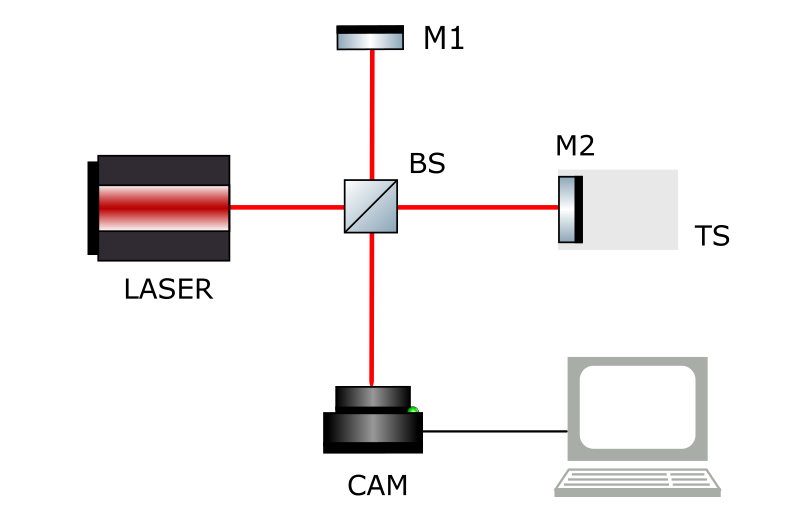
\includegraphics[width=0.55\linewidth]{figures/michelsoninkscape.png}
    \caption{Schematic Representation of Michelson interferometer used for displacement measurements with camera detection.  BS denotes the beam splitter, M1 the reference mirror, M2 the measurement mirror, TS the translation stage, and CAM the camera.}
    \label{fig:interferometer_setup}
\end{figure}

\begin{figure}[htbp]
    \centering
    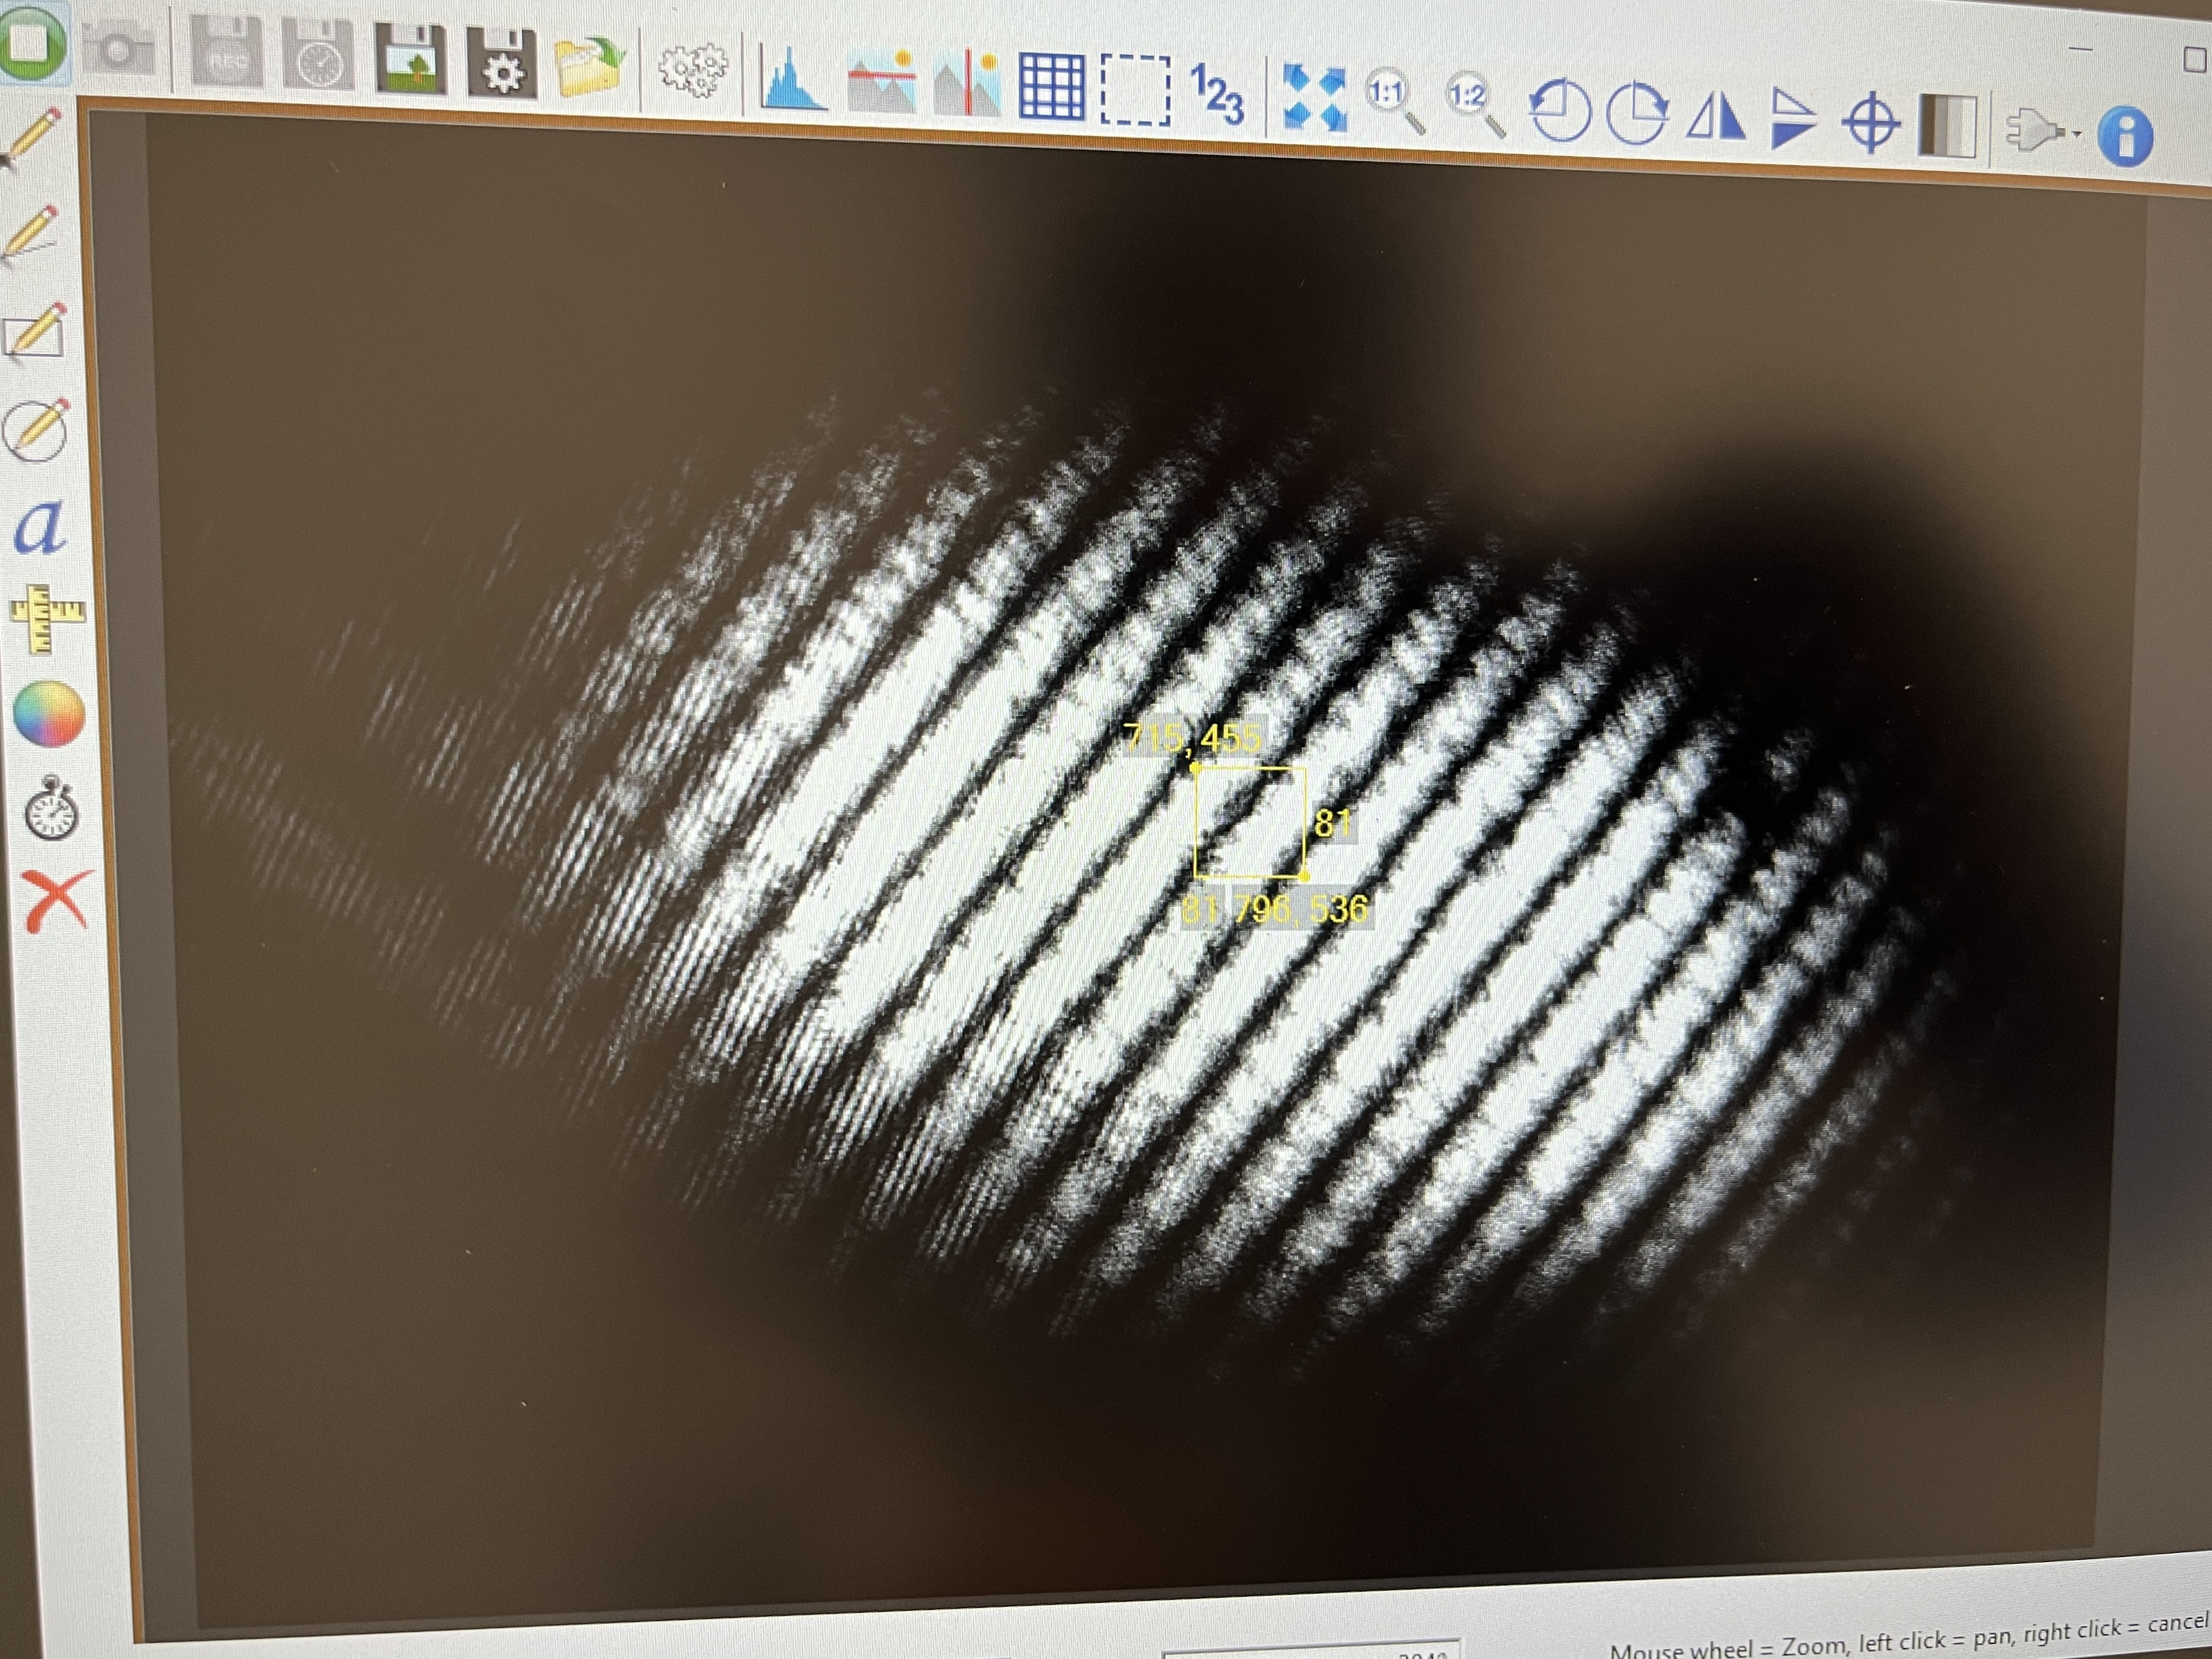
\includegraphics[width=0.5\linewidth]{figures/fringes_thorcam.jpg}
    \caption{Stable interference fringes observed with the camera in the ThorCam software.}
    \label{fig:thorcam_fringes}
\end{figure}

The stability and visibility of the observed interference pattern indicated that image-based fringe detection was a promising approach. Consequently, the development of dedicated software for automated fringe detection and fringe counting was considered feasible.

\subsection{Comparison with the Best HeNe Laser Source}

As discussed in Chapter 3, the Thorlabs diode laser exhibited the most stable intensity profile and was therefore mainly used for the interferometric measurements. To compare its performance with a HeNe source, the camera-based fringe detection measurement described above was repeated using the Uniphase 1023P HeNe laser. This laser was selected because it showed the best intensity stability among the investigated HeNe sources, which was considered the most important criterion for reliable fringe detection.

The experimental setup and evaluation procedure were kept unchanged; only the laser source was replaced. Compared with the diode laser, the fringe motion was less clearly detectable when using the HeNe laser. In contrast, the diode laser produced fringes with sharper edges and higher temporal stability, which made the fringe motion easier to identify reliably. The corresponding camera-based evaluation result for the HeNe laser is shown in Figure~\ref{fig:best_hene_cam_result}.

\begin{figure}[htbp]
    \centering
    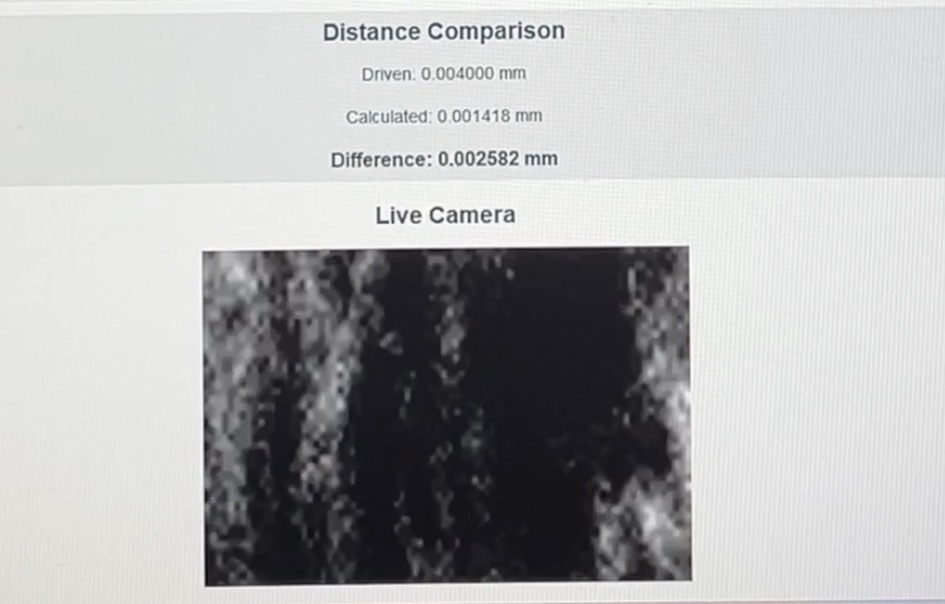
\includegraphics[width=0.8\linewidth]{figures/besthenecamresult.jpg}
    \caption{Camera-based fringe detection result obtained with the Uniphase 1023P HeNe laser.}
    \label{fig:best_hene_cam_result}
\end{figure}



\section{Electronic Signal Detection}

As an alternative to image-based fringe detection, an electronic detection approach was investigated. In this configuration, the optical output of the interferometer was directed onto a photodiode, converting the optical intensity variations into an electrical signal. The resulting signal was analyzed using a National Instruments USB-6221 data acquisition device. The experimental setup is shown in Figure~\ref{fig:photodiode_setup}.

\begin{figure}[htbp]
        \centering
        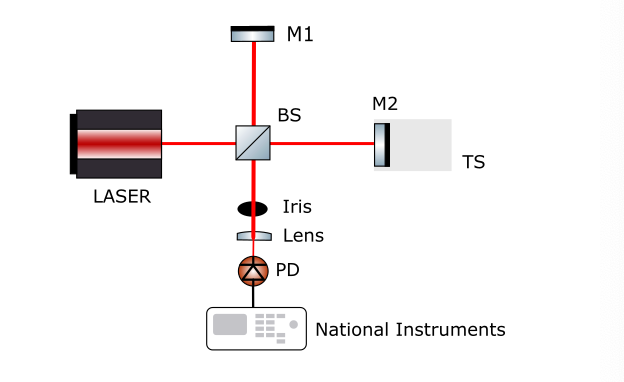
\includegraphics[width=0.75\linewidth]{figures/electronicsignalschematic.png}
    \caption{Electronic signal detection using a photodiode, schematic representation. BS denotes the beam splitter, M1 the reference mirror, M2 the measurement mirror, TS the translation stage, and PD the photodiode.}
    \label{fig:photodiode_setup}
\end{figure}

In principle, displacement of the translation stage should produce periodic intensity variations in the interference signal, with destructive interference corresponding to intensity minima and constructive interference corresponding to intensity maxima.  

During these measurements, the PI translation stage described at the beginning of this chapter was temporarily unavailable. Therefore, a Thorlabs LTS300C/M translation stage was used instead. The control software was adapted accordingly to drive the Thorlabs stage. Since only the stage actuation was changed while the interferometric detection principle remained the same, the results can still be compared with the camera-based diode laser measurements.
       
With these modifications, fringes could also be detected from the electronic photodiode signal. The corresponding result is shown in Figure~\ref{fig:electronic_signal_detection}.

\begin{figure}[htbp]
    \centering
    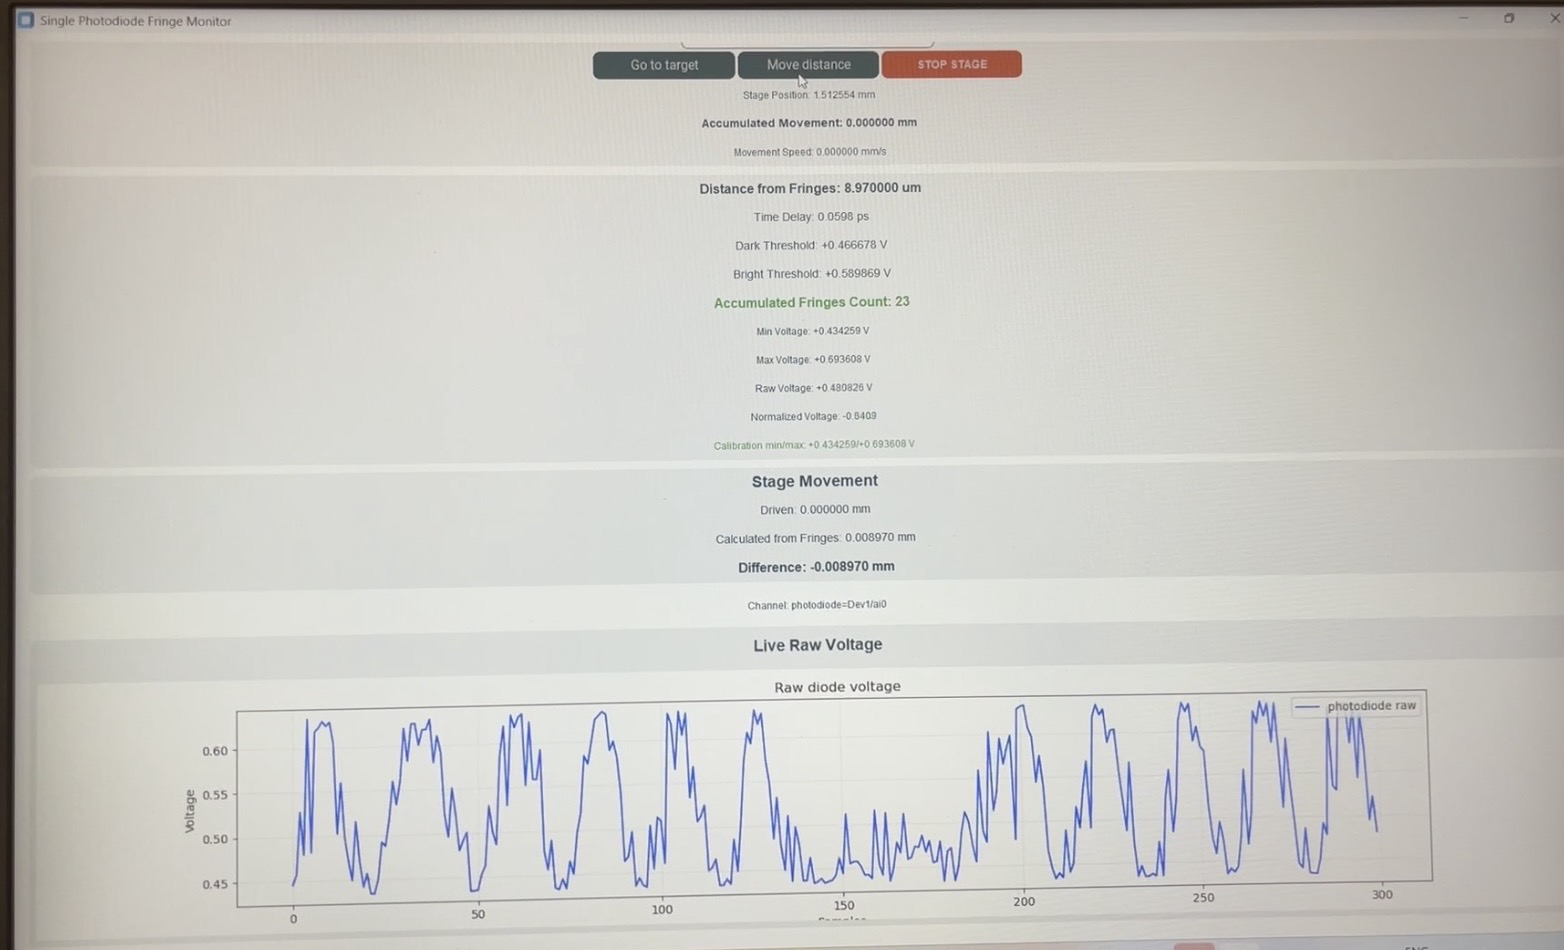
\includegraphics[width=0.8\linewidth]{figures/electronicsignaldetection.jpg}
    \caption{Fringe detection result obtained from the electronic photodiode signal.}
    \label{fig:electronic_signal_detection}
\end{figure}

\section{Comparison of Detection Methods}

The two investigated detection approaches showed a different performance levels. The camera provided stable and clearly visible interference fringes with a high signal-to-noise ratio, enabling robust image-based evaluation. Furthermore, the recorded fringe patterns offered direct visual feedback during alignment and facilitated the development of automated analysis software.

The photodiode-based detection approach also produced a usable periodic signal. One advantage of this method is that the sinusoidal intensity variation can be monitored directly in the voltage signal. This makes missed fringes or undetected peaks easier to identify than in camera-based detection, where fringes may become difficult to distinguish during rapid motion. However, the photodiode signal was not consistently stable. In some intervals, the sinusoidal modulation flattened or shifted, and the number of visible fringes varied over comparable time periods. These observations indicate that the signal-to-noise ratio and baseline stability were not sufficient for the highest measurement accuracy.

Unfortunately, the absolute measurement accuracy of the camera- and photodiode-based methods cannot be compared quantitatively. Such an analysis would require a reference system with a significantly higher accuracy, for example a calibrated interferometer or a translation stage whose displacement is known with negligible uncertainty. Neither of these was available in this work.

Using the translation stage as the reference would not be appropriate, since the purpose of the developed interferometer is precisely to characterize and improve the stage's positioning accuracy. Any uncertainty in the stage motion would therefore directly affect the calculated measurement uncertainty, resulting in a circular validation.

Therefore, the two methods were compared in terms of their repeatability rather than their absolute accuracy. The translation stage was commanded to perform the same nominal displacement of \(0.5\,\mathrm{mm}\) repeatedly, first using the camera-based system and then the photodiode-based system. The resulting fringe counts and calculated displacements were evaluated by comparing their standard deviations. Although this approach does not provide the absolute measurement error of either method, it allows their measurement repeatability to be assessed under identical experimental conditions and represents the most meaningful comparison that could be performed with the available experimental setup.

The repeatability comparison is shown in Figure~\ref{fig:fringe_summary_combined}. Across the three repeated measurements, the camera-based evaluation showed a slightly smaller variation in the calculated displacement than the photodiode-based evaluation. However, because only three measurements were performed, this difference cannot be considered statistically significant. Instead, the results indicate that both methods were able to reproduce the commanded displacement reliably under the investigated conditions.

\begin{figure}[htbp]
    \centering
    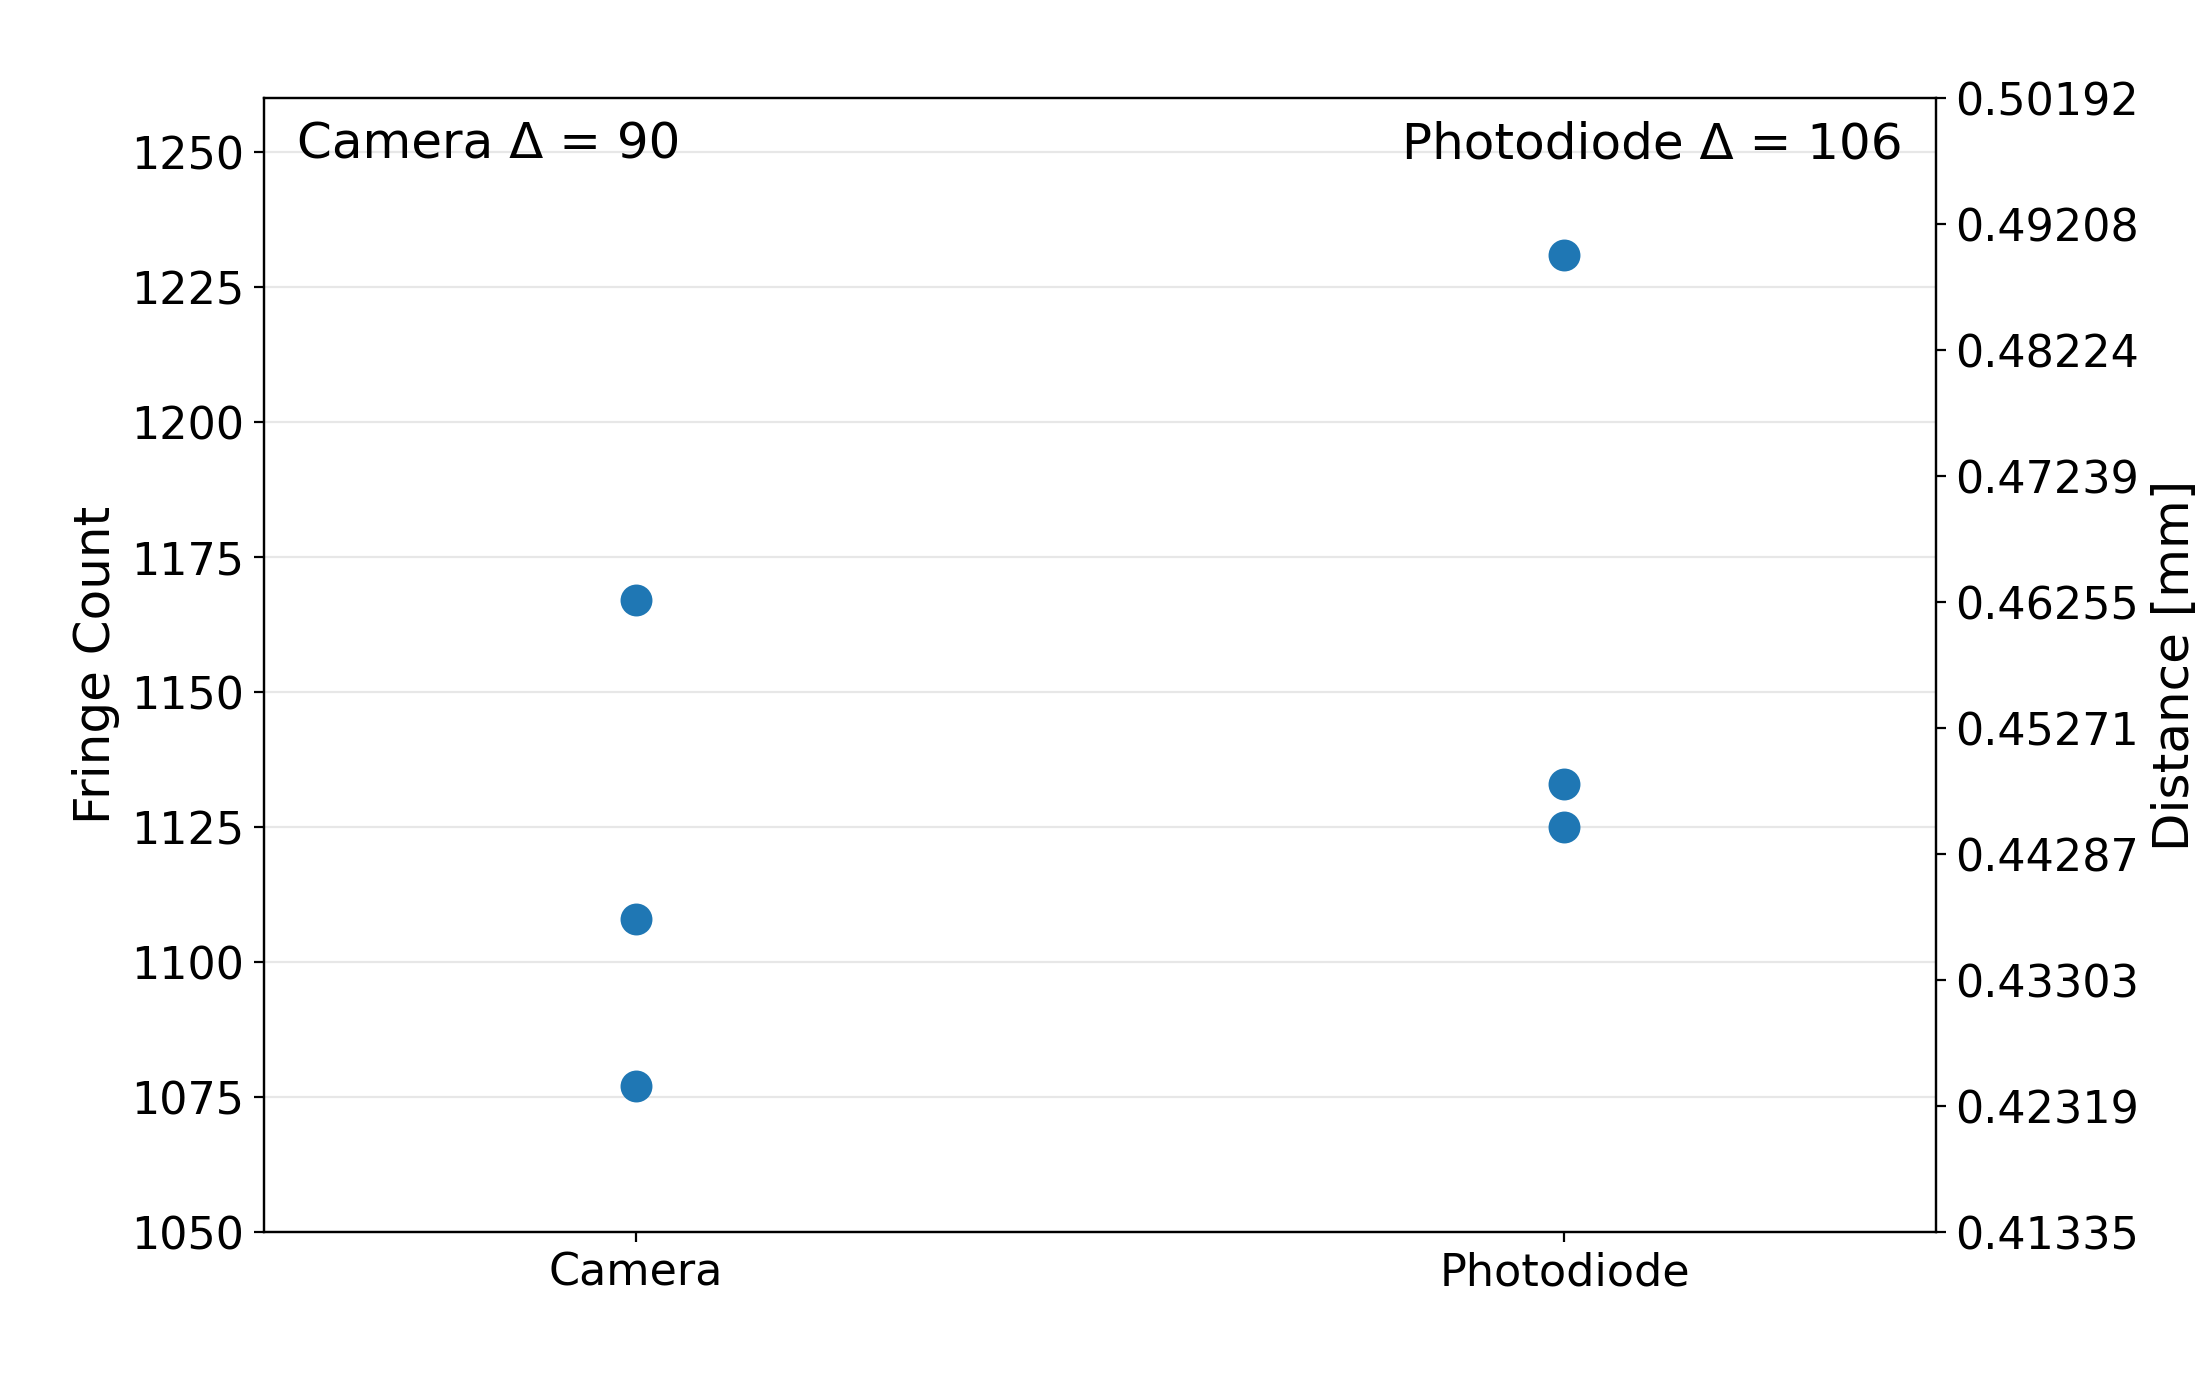
\includegraphics[width=0.8\linewidth]{figures/fringe_summary_combined.png}
    \caption{Comparison of the calculated displacements obtained from camera-based and photodiode-based fringe detection for repeated nominal displacements of \(0.5\,\mathrm{mm}\).}
    \label{fig:fringe_summary_combined}
\end{figure}

A more noticeable difference can be seen in Figure~\ref{fig:camera_diode_side_by_side}. The camera-based signal was less affected by environmental noise and short-term disturbances, while the photodiode signal showed larger fluctuations and variations in the baseline.  Although the repeatability measurements did not show a significant difference between the two methods, the camera-based approach provided a more stable signal under the investigated conditions.

\begin{figure}[htbp]
    \centering
    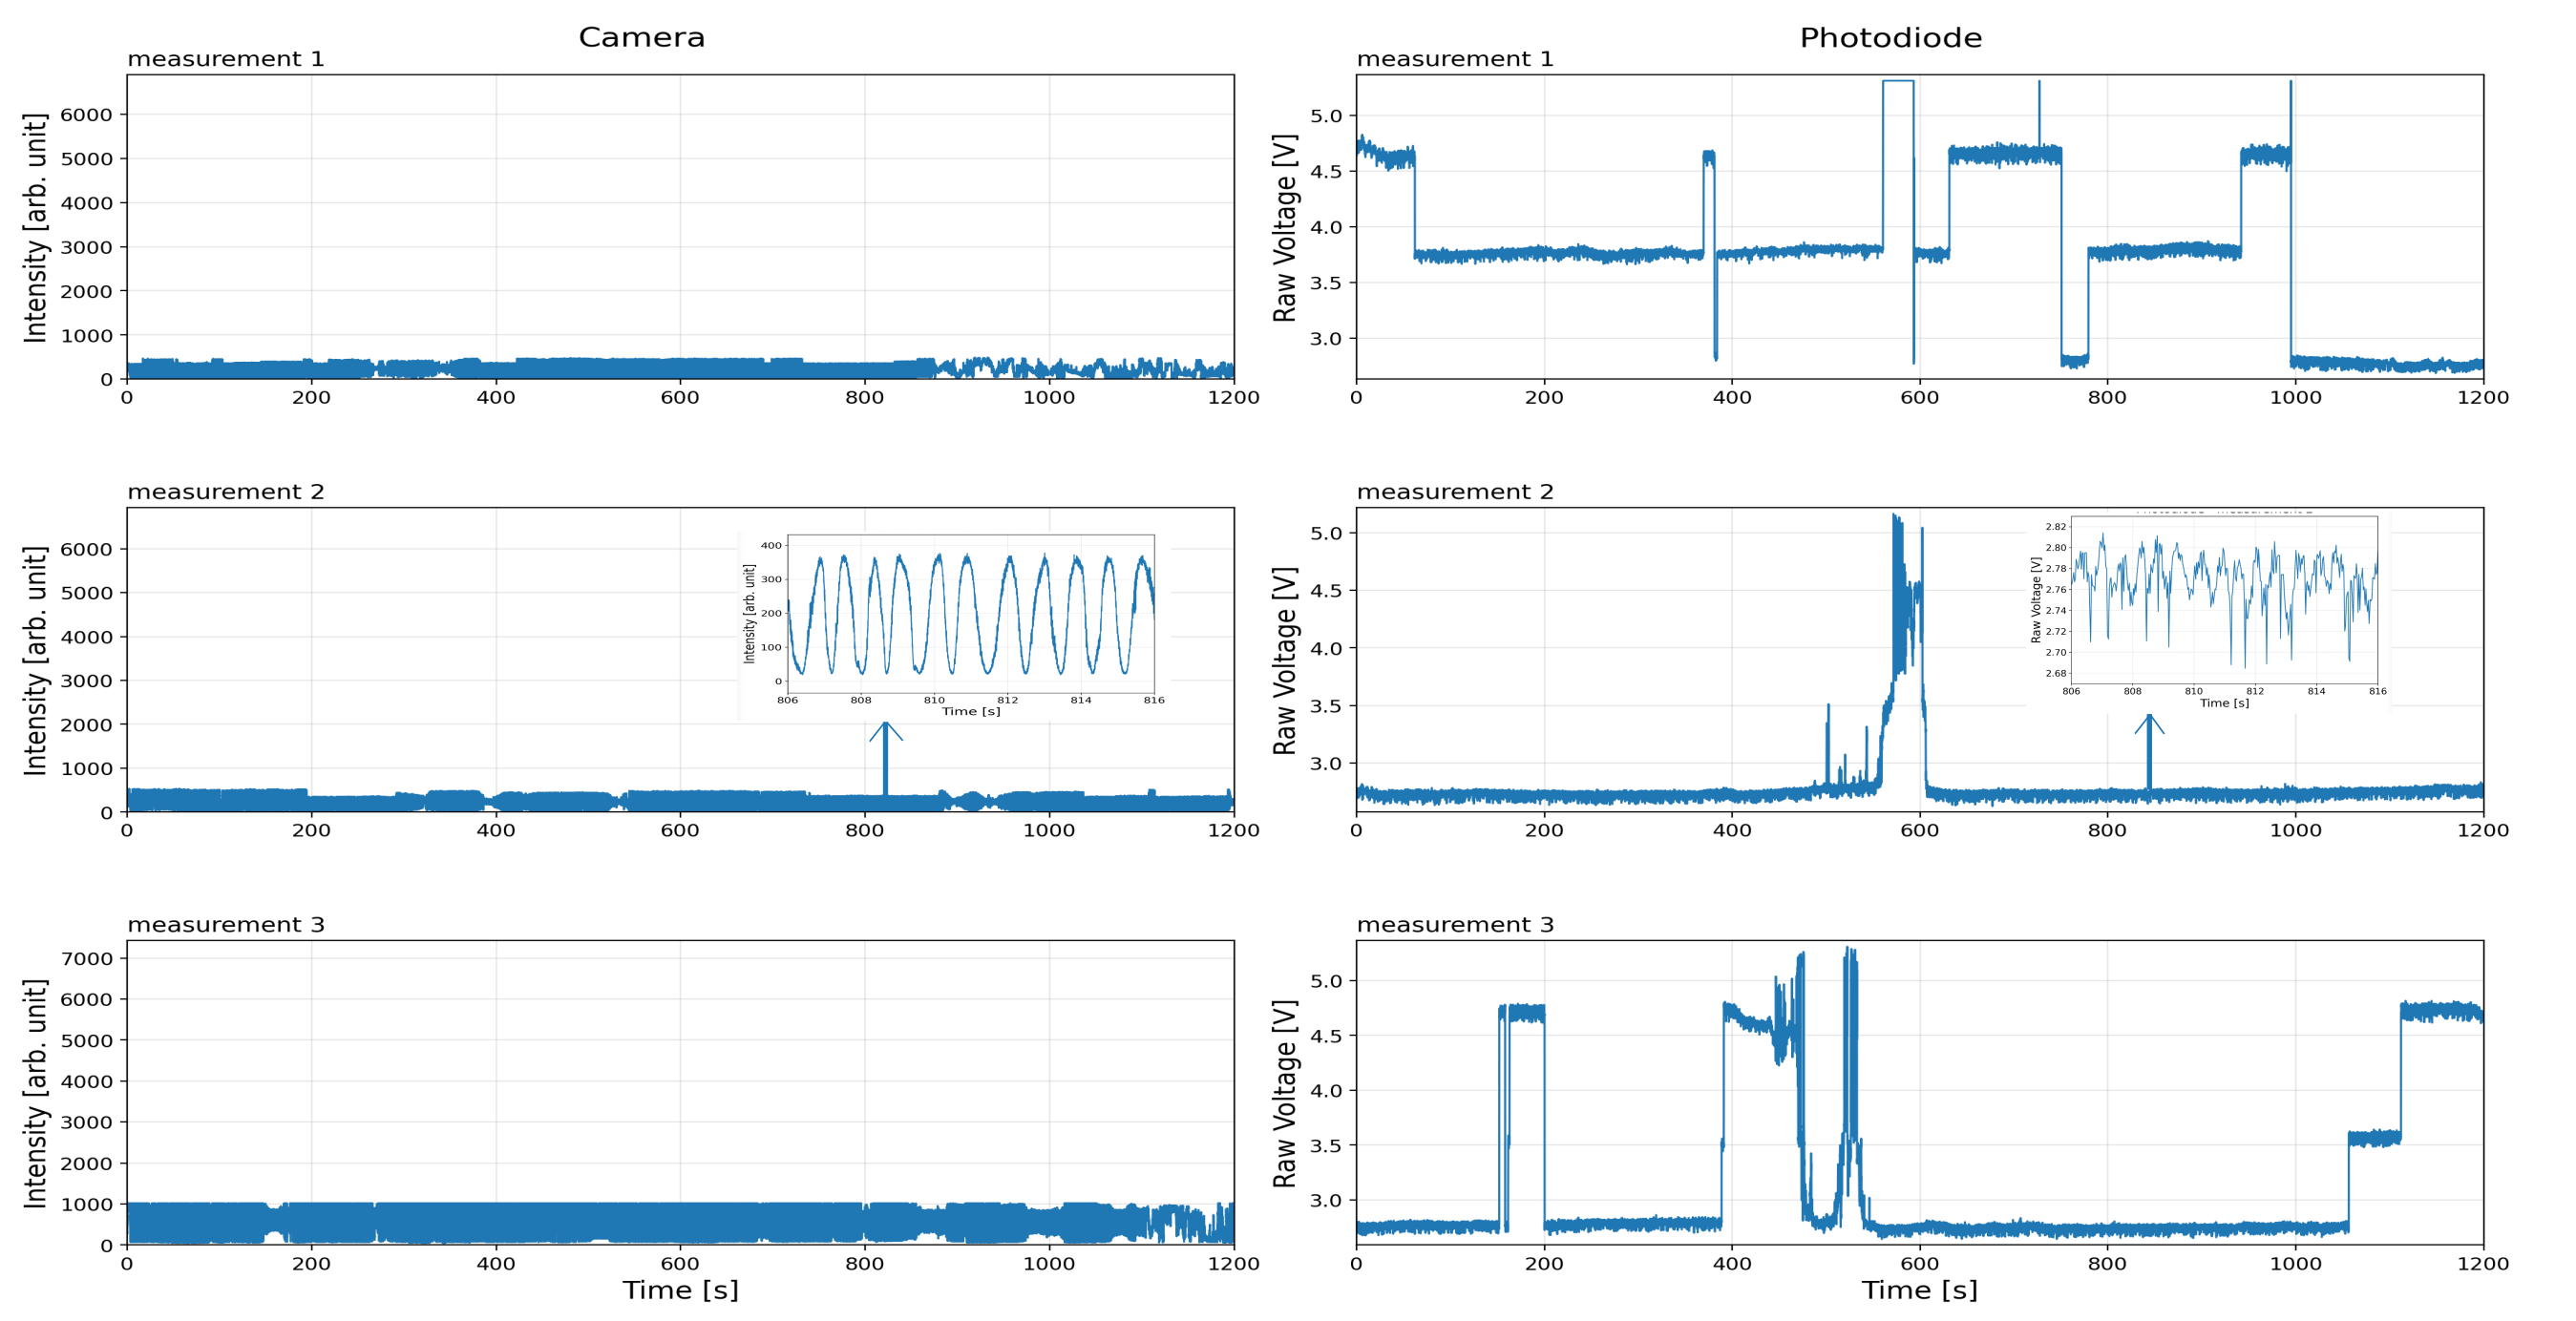
\includegraphics[width=1.0\linewidth]{figures/camera_diode_side_by_side.png}
    \caption{Side-by-side comparison of camera-based and photodiode-based fringe detection. The camera-based evaluation is less affected by environmental noise, while the photodiode signal exhibits stronger fluctuations. The camera-based measurement was performed at a stage velocity of \(0.0004\,\mathrm{mm\,s^{-1}}\), whereas the photodiode-based measurement was performed at \(0.0006\,\mathrm{mm\,s^{-1}}\). For clearer visualization, both datasets are shown only up to \(1200\,\mathrm{s}\), although the camera-based measurement contained additional data. This time interval was sufficient for comparing the signal stability of both detection methods.}
    \label{fig:camera_diode_side_by_side}
\end{figure}

During the experimental work, additional limitations of the diode laser became apparent. It showed noticeable variations between repeated measurements. In addition to differences between individual measurements, the signal quality also varied from one day to another.

Another observation was that the interference signal occasionally required a short settling time before stable fringes appeared. In these cases, the translation stage had already started moving, while the interference fringes became visible only after a short delay. The reason for this behaviour could not be identified within the scope of this thesis.

Overall, the system did not provide the same signal quality under all measurement conditions. If the setup is used in future experiments, it should be operated in a better isolated environment to reduce the influence of air currents, vibrations of the optical table, and other external disturbances. Due to the limited scope and timeframe of this thesis, implementing these improvements was not possible. 



\section{Quadrature Homodyne Interferometer}
As discussed in the introduction, the interferometer was not only intended to improve the accuracy of the translation stage displacement measurement. A second important requirement was the detection of the direction of motion, since small forward and backward movements of the stage in a stationary position must be compensated for in order to enable active correction. For this reason, the Michelson interferometer was extended with polarization optics to form a quadrature homodyne interferometer. The corresponding laboratory setup and schematic representation are shown in Figure~\ref{fig:quadrature_homodyne_setup}.

\begin{figure}[htbp]
    \centering
    \begin{minipage}[t]{0.48\linewidth}
        \centering
        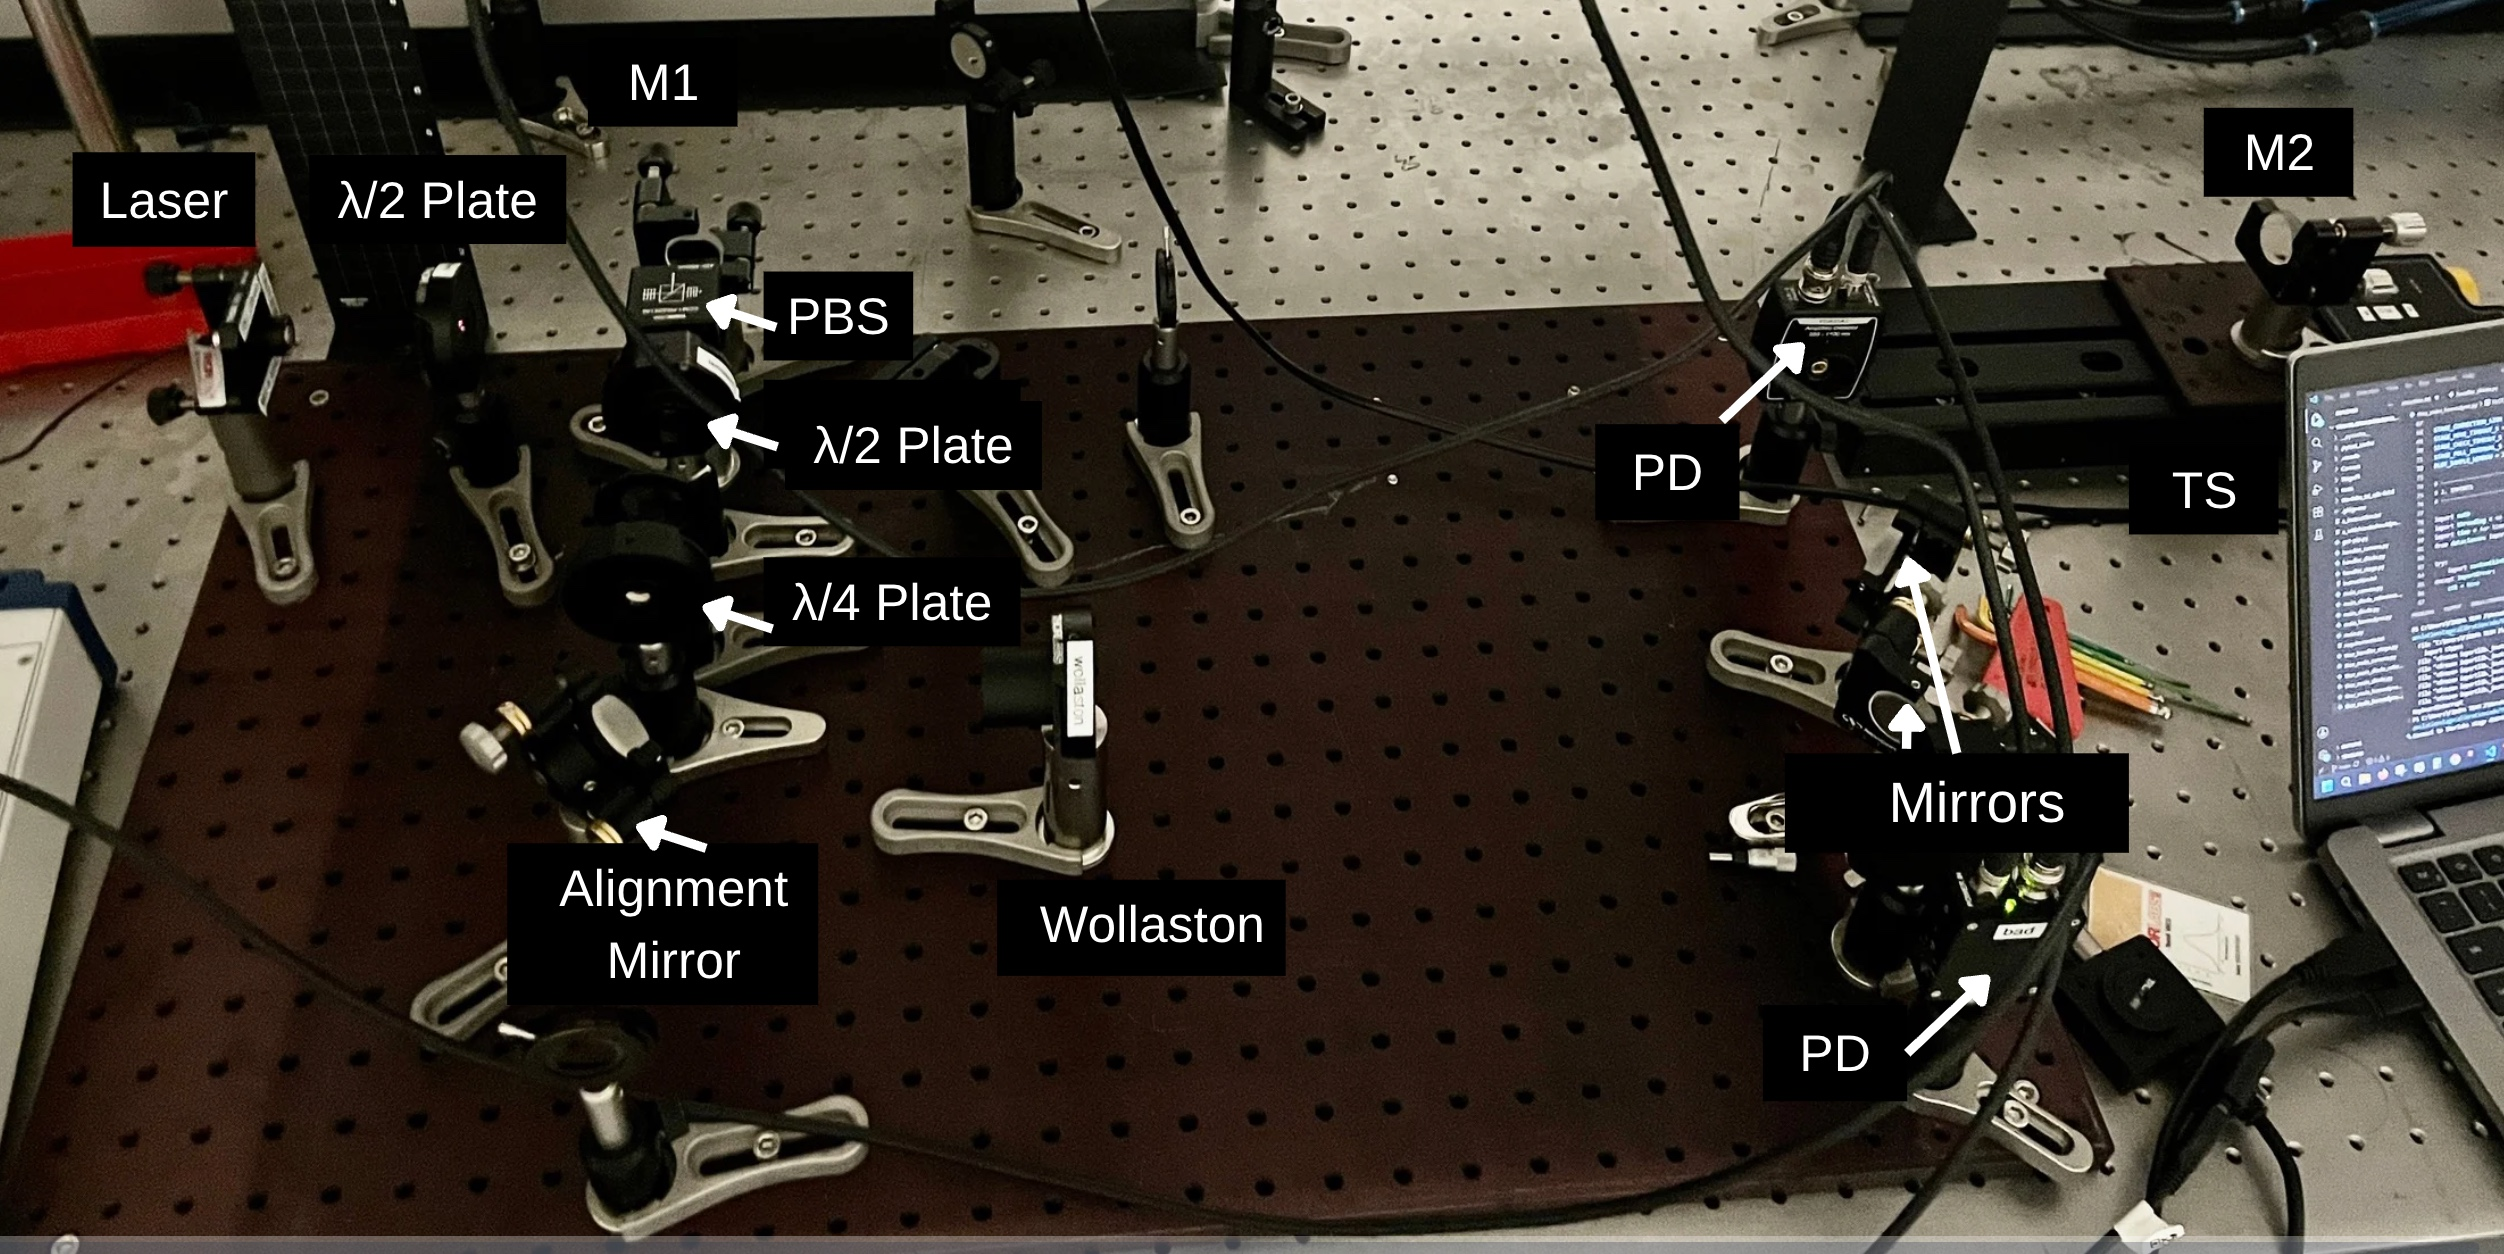
\includegraphics[width=\linewidth]{figures/homodynesetuplab.jpeg}
    \end{minipage}\hfill
    \begin{minipage}[t]{0.48\linewidth}
        \centering
        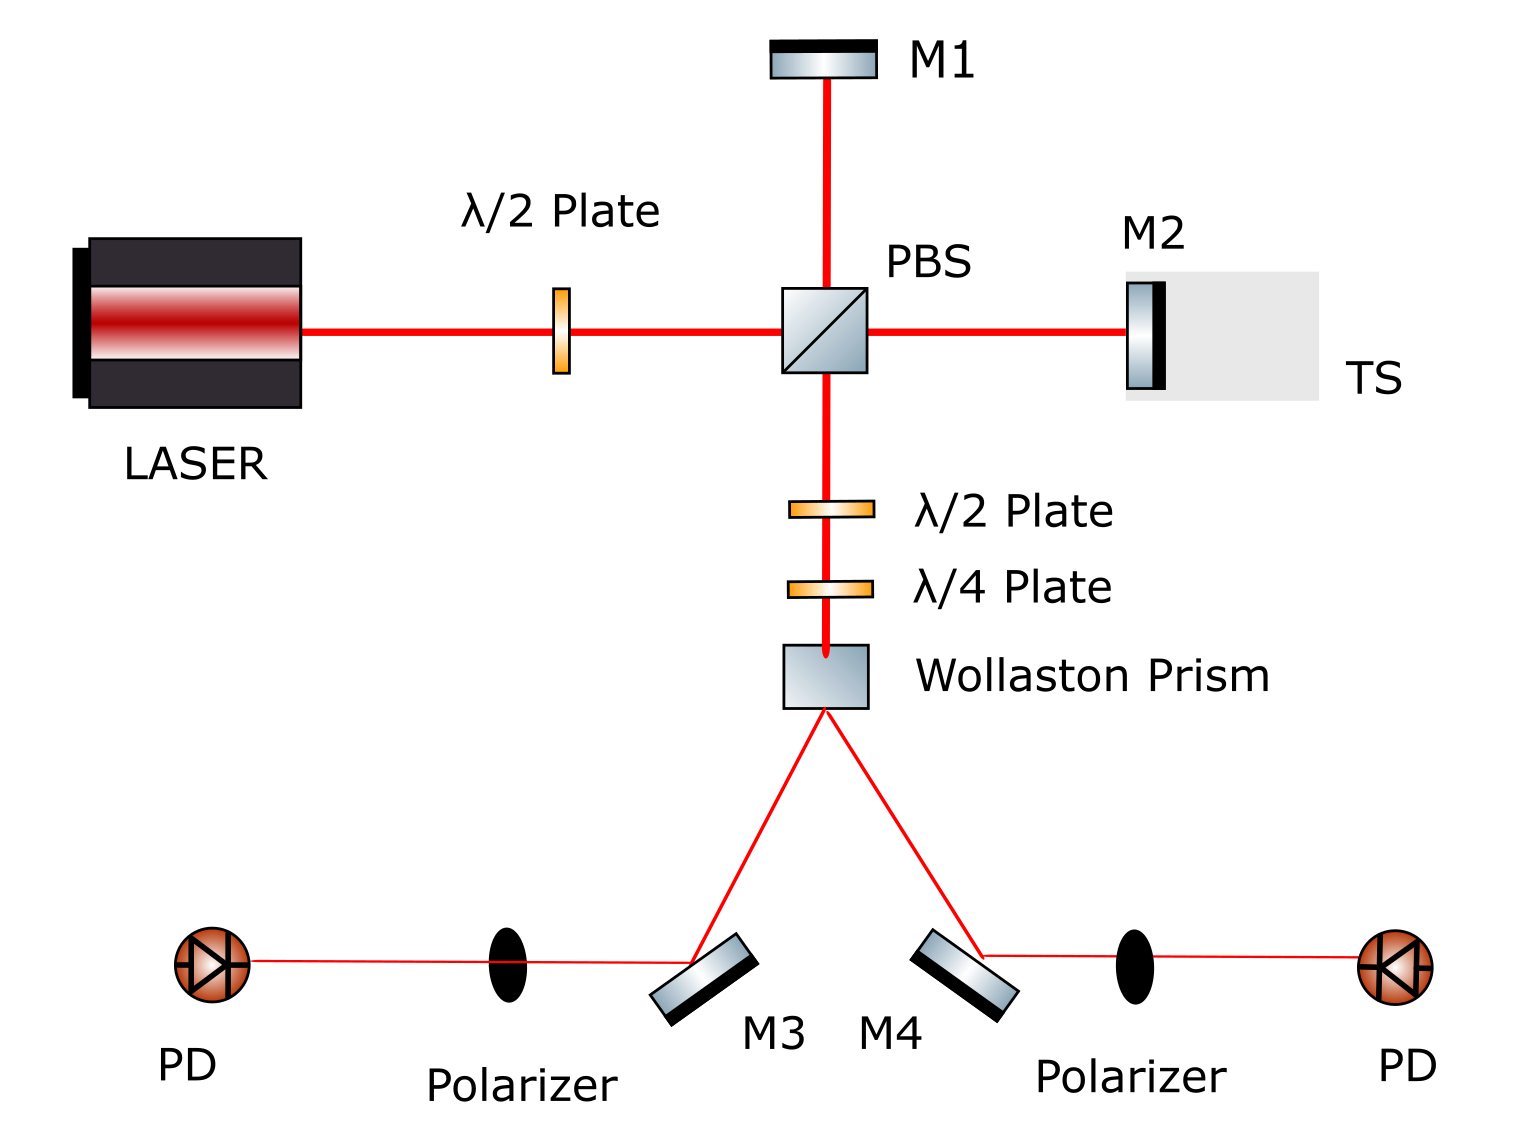
\includegraphics[width=\linewidth]{figures/homodyneschematic.png}
    \end{minipage}
    \caption{Laboratory setup and schematic representation of the quadrature homodyne interferometer. The setup extends the Michelson interferometer with polarization optics in order to generate two phase-shifted photodiode signals for direction-sensitive displacement detection. M1--M4 denote mirrors, PD denotes the photodiode, TS denotes the translation stage, and PBS denotes the polarizing beam splitter. Although the polarizers at the end are included in the schematic for completeness, they are omitted in the actual setup photograph, as the Wollaston prism theoretically acts as a perfect polarizing beam splitter.}
    \label{fig:quadrature_homodyne_setup}
\end{figure}

In this configuration, the laser beam first passes through a half-wave plate, which rotates the linear polarization to \(45^\circ\). The beam then enters a polarizing beam splitter, where it is ideally divided into equal s- and p-polarized components. These two components form the two interferometer arms and are reflected by mirrors. Due to the temporary unavailability of the PI translation stage, these measurements were also performed using the Thorlabs LTS300C/M translation stage.

After propagating through the interferometer arms, the two beams are recombined and pass through a second half-wave plate. This wave plate rotates the polarization by \(45^\circ\), so that both beams contain equal amounts of s- and p-polarized light. The beams then pass through a quarter-wave plate, which introduces a phase shift of \(\pi/2\) between the two polarization components and converts the light into circularly polarized light. This allows the Wollaston prism to generate two interference signals that are \(90^\circ\) out of phase, enabling quadrature detection. The Thorlabs MgF2 (10mm thickness) Wollaston prism acts as a polarization beam splitter and generates two output beams with orthogonal polarization components. These beams are redirected by two mirrors and then pass through polarizers to clean up the respective polarization states before detection with a photodiode.

The polarization states in the quadrature homodyne interferometer are illustrated schematically in Figure~\ref{fig:homodyne_polarization}. This representation clarifies how the polarization optics generate two detection signals with an approximate phase shift of \(90^\circ\).

\begin{figure}[htbp]
    \centering
    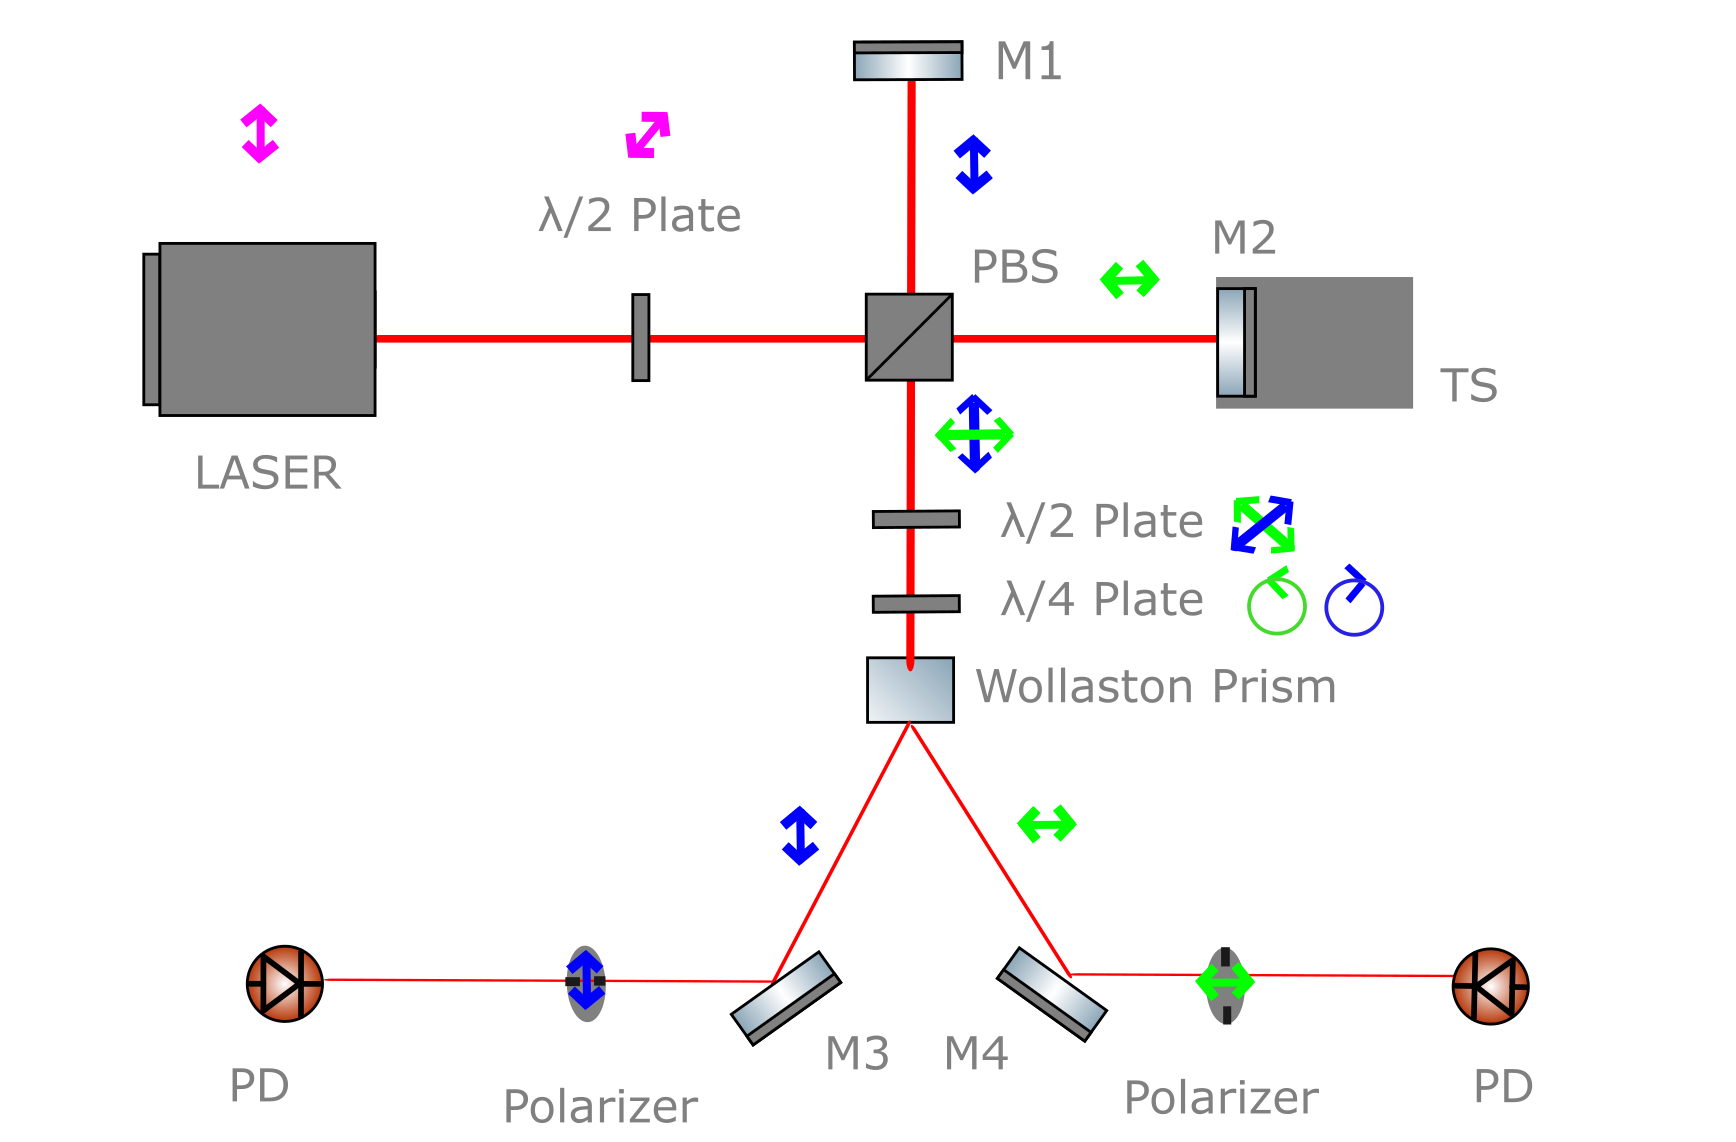
\includegraphics[width=0.8\linewidth]{figures/homodynepol.png}
    \caption{Schematic representation of the polarization states in the quadrature homodyne interferometer. M1--M4 denote mirrors, PD denotes the photodiode, TS the translation stage, and PBS the polarizing beam splitter.}
    \label{fig:homodyne_polarization}
\end{figure}

The two phase-shifted photodiode signals were successfully detected. The direction of motion can be determined from the Lissajous plot shown on the right-hand side of the graphical user interface (see Figure~\ref{fig:homodyne_software_gui} in Chapter~\ref{chap:software_analysis}). The two quadrature signals form a circular trajectory, and the direction in which this trajectory is moving indicates the direction of motion.

A detailed evaluation of the recorded quadrature signals is shown in Figure~\ref{fig:sin_cos_fit}. One photodiode signal was fitted with a sine function, while the second signal was fitted with a cosine function. The fitted curves show a phase shift of \(90^\circ\), as indicated by the dashed vertical reference line passing through corresponding points of the two fitted signals. This confirms that the optical setup generated the required quadrature phase relation for direction-sensitive displacement detection.

\begin{figure}[htbp]
    \centering
    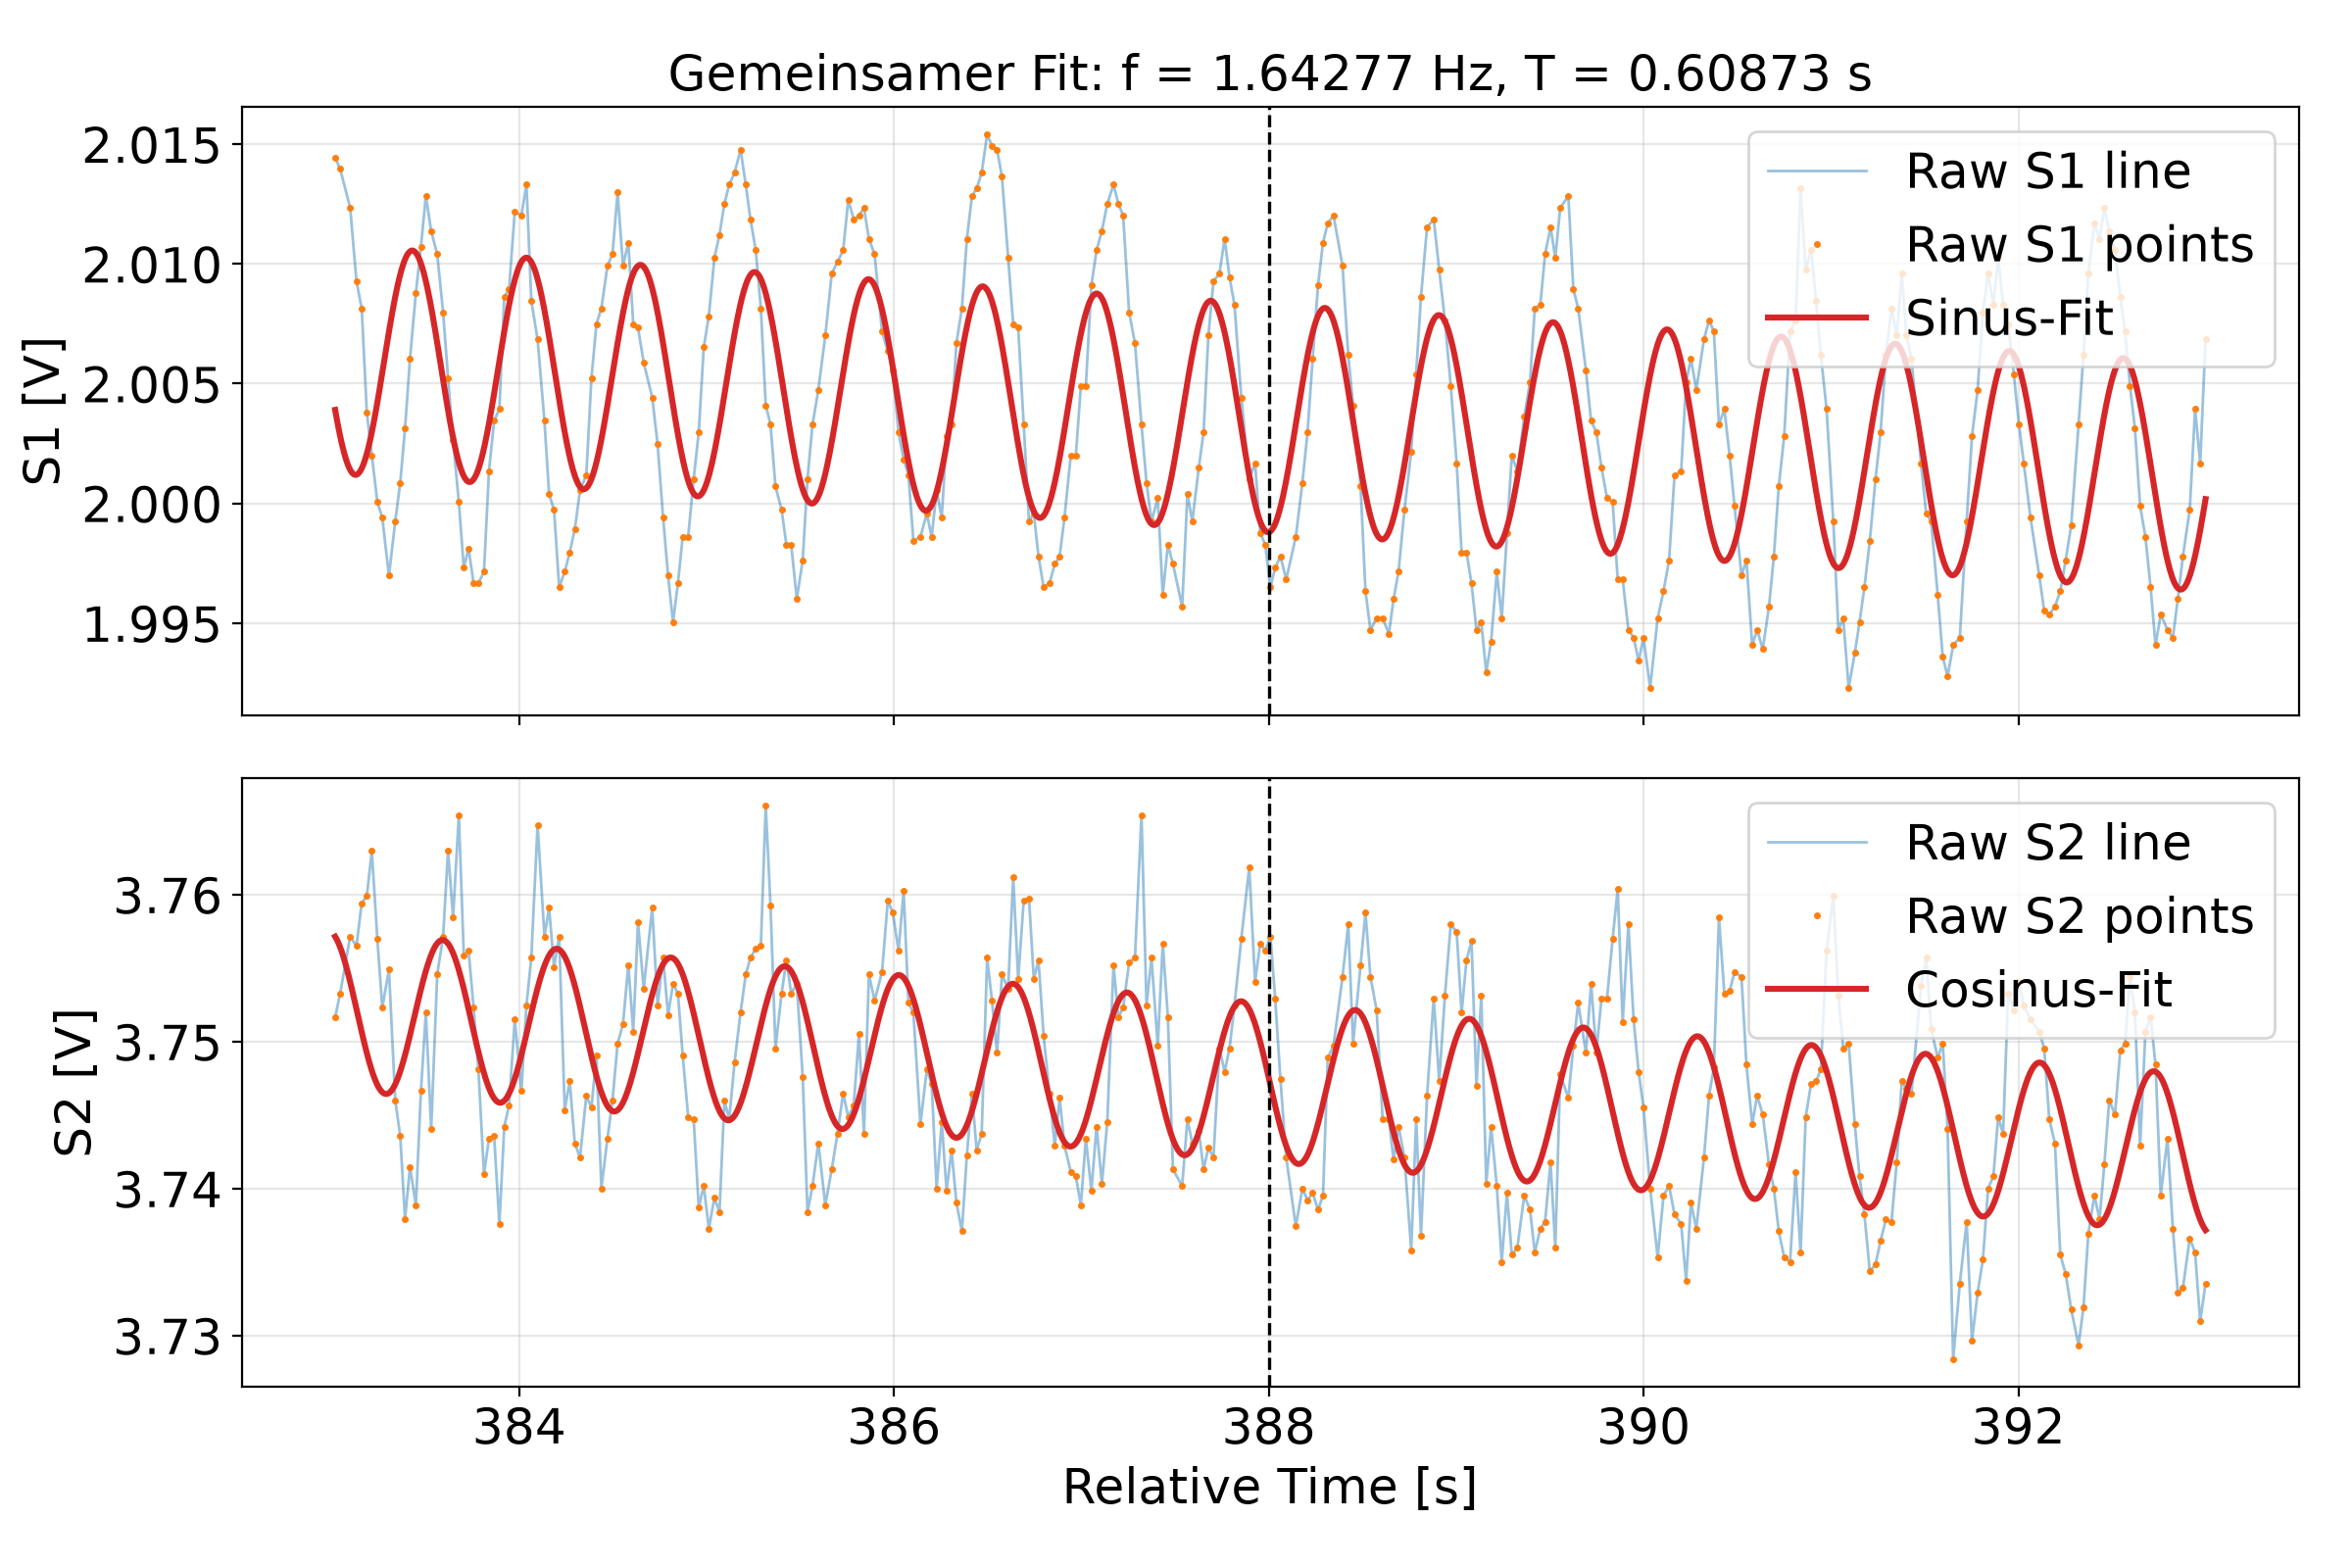
\includegraphics[width=0.8\linewidth]{figures/sin_cos_fit.png}
    \caption{Detailed evaluation of the quadrature homodyne signals. The fitted sine and cosine curves show a phase shift of \(90^\circ\), confirming the quadrature relation between the two photodiode signals.}
    \label{fig:sin_cos_fit}
\end{figure}

To verify that the quadrature homodyne interferometer can determine the direction of motion over longer travel distances, the translation stage was moved repeatedly over a distance of \(0.5\,\mathrm{mm}\). This distance was chosen to be consistent with the comparison of the camera- and photodiode-based detection methods. At a stage velocity of \(0.0006\,\mathrm{mm\,s^{-1}}\), this displacement corresponds to a comparatively long measurement time and therefore provides a useful test of the stability of the direction detection.

The stage was moved three times in the forward direction and three times in the backward direction. During each measurement, the software assigned every recorded data point to one of the three states \textit{forward}, \textit{backward}, or \textit{still}. The resulting percentages are summarized in Table~\ref{tab:homodyne_direction_validation}.

\begin{table}[htbp]
    \centering
    \caption{Direction classification obtained with the quadrature homodyne interferometer during repeated \(0.5\,\mathrm{mm}\) stage movements.}
    \label{tab:homodyne_direction_validation}
    \begin{tabular}{lccc}
        \hline
        Commanded motion & Forward (\%) & Backward (\%) & Still (\%) \\
        \hline
        Backward 1 & 18.93 & 63.82 & 17.25 \\
        Backward 2 & 17.08 & 66.27 & 16.65 \\
        Backward 3 & 12.68 & 70.79 & 16.54 \\
        Forward 1  & 67.01 & 13.08 & 19.91 \\
        Forward 2  & 63.94 & 17.82 & 18.24 \\
        Forward 3  & 78.55 & 8.22  & 13.23 \\
        \hline
    \end{tabular}
\end{table}

For all six measurements, the largest fraction of data points corresponds to the commanded direction of motion. This shows that the quadrature homodyne interferometer was able to detect the direction correctly. However, a noticeable fraction of the data points was classified as \textit{still} or as the opposite direction. This is mainly attributed to noise and signal instabilities. Therefore, the measurement confirms the general functionality of the direction detection, while also showing that further optimization of the signal quality would improve its robustness.


